\section{簡介}
在上一章中,我們嘗試了使用聲學片段加強語意檢索的成果,使得系統能夠在接收到文字形式的查詢詞後,進行語意檢索回傳給使用者語意相關的語音文件。這系統仍然需要一套被訓練好的辨識系統才能發揮功效,但是訓練辨識系統中的聲學模型和語言模型都需要很大量的人工標注資料,要得到這些資料往往是很昂貴的,因此近年來「非監督式學習」(Unsupervised Learning) 逐漸成為學術界關注的焦點,原因是全世界每天產生很大量的語音與文字資料,取得未標注的資料是很容易的事,再加上近年大數據 (Big Data)
風潮使得許多公司與學術單位開始學習如何分析大數據,並從數據中汲取有用的資料,因此非監督式學習試圖直接從未標注的語音文件中找出規律,並且在不需要大量的人為標注下達成目標。

過去幾乎所有的非監督式方法都是實作在口述語彙偵測 (系統只回傳包含查詢詞的文件) 上的,而完全沒有實作在語意檢索上。但使用者通常不會只想找到包含查詢詞的文件,使用者想找的是與查詢詞最「語意相關」的文件,因此本章試圖提出基於相關回饋的新方法:系統會先利用將所有的語音文件辨識成上一章提到的聲學片段序列,當使用者「口述」一句查詢詞給系統後,系統會使用動態時間扭曲 (Dynamic Time Warping, DTW) 按照語音文件中是否有出現此句查詢詞排序後產生第一次檢索結果,並假設第一次檢索結果的前$N$篇為虛擬相關文件,再將虛擬相關文件中很常一起出現的聲學片段當作和查詢詞語意相關的詞彙並將其當作新的查詢詞模型用作查詢詞擴展。
  
\section{使用動態時間扭曲之口述語彙偵測}
\label{sec:chap4_sdtw}
口述語彙偵測的目的是要搜尋整個語料庫後,找出其中有出現查詢詞的語音文件,並且找出這些語音文件中可能有出現查詢詞的假定區域 (Hypothesis Region) ,並給這個假定區域一個相關分數,最後系統再根據相關分數進行排序後回傳給使用者 (分數較高為較相關)。

這裡使用的口述語彙偵測方法為片段動態時間扭曲 (Segmental Dynamic Time Warping)~\cite{chan2010unsupervised, hazen2009query}。假設輸入的查詢詞的特徵為$\mathbf{X} = (\mathbf{x}_1, ..., \mathbf{x}_{|\mathbf{X}|}$,語音文件的特徵為$\mathbf{Y} = (\mathbf{y}_1, ..., \mathbf{y}_{|\mathbf{Y}|})$,有了這兩者之後,就可以建立一個距離表格 (Distance Table) $D(i, j) = \rho(\mathbf{x}_i, \mathbf{y}_j)$,通常這裡使用的特徵是
% TODO 
高斯事後機率 (Gaussian Posteriorgrams)~\cite{zhang2009unsupervised},而兩個音框之間的距離為 $\rho(\mathbf{x}, \mathbf{y}) \equiv -\log (\mathbf{x}, \mathbf{y})$。

動態時間扭曲的目的是要在 $D(i, j)$ 上找一條總合最短的路徑從 $(1, s)$ 到 $(|\mathbf{X}|, e)$ 表示從 $\mathbf{X}$對應到$(\mathbf{y}_s, ..., \mathbf{y}_e)$ (因為查詢詞一定要被完全對應,而語音文件不一定要被完全對應到)。由於假定區域可以出現在語音文件中的任何地方, 因此片段動態時間扭曲將距離表格 $D(i, j)$ 切成數個重疊的對角片段 (寬度為 $R$),所以說每個片段的起始點分別為 $(1, 1), (1, 1+R), (1, 1+2R),...$ 如圖 ~\ref{fig:chap4_sdtw} 所示,每個對角片段都代表了一個可能出現查詢詞的區域,即一個假定區域。片段動態時間扭曲會從每個片段中找出一段距離總合最短的路徑,在每個片段中所有對應的路徑 (Warping Path) 都必須要完整地待在片段內,不可超出片段。

\begin{figure}
\centering
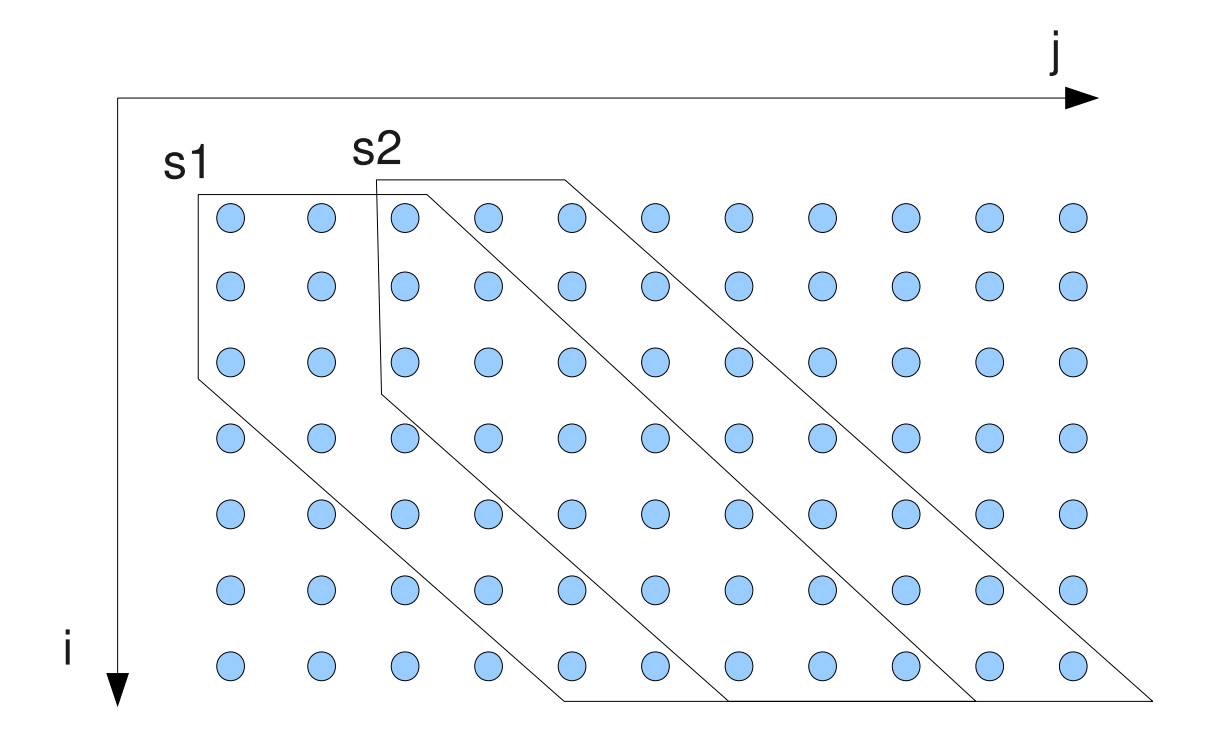
\includegraphics[scale=0.3]{images/chap4_sdtw.png}
\caption{片段動態時間扭曲示意圖~\cite{zhang2009unsupervised}} \label{fig:chap4_sdtw}
\end{figure}

假設在每個片段中的對應路徑為:

\[
\phi = (i_t, j_t), t = 1,...,|\phi|
\]

代表著如下的對應關係:

\[
\mathbf{x}_{i_1} \leftrightarrow \mathbf{y}_{j_1}, \mathbf{x}_{i_2} \leftrightarrow \mathbf{y}_{j_2},...,\mathbf{x}_{|\phi|} \leftrightarrow \mathbf{y}_{|\phi|},
\]
而邊界條件是 $i_1 = 1, i_{|\phi|} = |\mathbf{X}|$ ,$j_1$ 為 $1+kR$ ,對應路徑中所有的點都要在片段內,即:

\[
|(i_t-i_1)-(j_t-j_1)| <= R
\]

而片段動態時間扭曲的目標是要在每個片段內找到一條路徑 $\phi$ 使得下式的距離總和最小:

\begin{equation}
C_{\phi}(\mathbf{X}, \mathbf{Y}) = \sum_{t=1}^{|\phi|} \rho(\mathbf{x}_{i_t},\mathbf{y}_{j_t})
\end{equation}

每個片段中使得 $C_{\phi}(\mathbf{X}, \mathbf{Y})$ 最小,即使得相關分數 $-C_{\phi}(\mathbf{X}, \mathbf{Y})$ 最大的那條 $\phi$ 即為每個片段中的假定區域 $(\mathbf{y}_{j_1},...,\mathbf{y}_{j_{|\phi|}})$ ,而在每個片段中找到最大相關分數的路徑可以使用動態規劃 (Dynamic Programming) 求解。

\section{基於語音片段之語意檢索}
\subsection{系統架構}
系統架構如圖 ~\ref{fig:chap4_system},圖中的下半部為離線處理 (Offline Processing) 的部分,包括聲學片段的聲學模型、語言模型、辭典都是離線的時候自動從語料庫中學習出來的~\cite{chung2013unsupervised},有了聲學、語言模型和辭典後,即可用其建造出一個辨識系統 (圖~\ref{fig:chap4_system}中左下角) 將語音文件辨識成聲學片段形式的唯一最佳序列。圖~\ref{fig:chap4_system}中的上半部為在線處理 (Online Processing)
的部分,當使用者「口述」了一段查詢詞後,系統會使用片段動態時間扭曲 (在圖~\ref{fig:chap4_system}中的檢索引擎1) 產生第一次檢索結果,並假設其中最相關的前 $N$ 篇為虛擬相關,虛擬相關文件中時常出現的聲學片段即可視作是與查詢詞語意相關的聲學片段,這些即為擴展後的查詢詞模型,接下來圖中的檢索引擎2 會利用擴展後查詢詞模型尋找之前得到的聲學片段形式的唯一最佳序列,如果這些唯一最佳序列中包含了這些與查詢詞語意相關的聲學片段,即是與原查詢詞語意相關的文件。

\begin{figure}
\centering
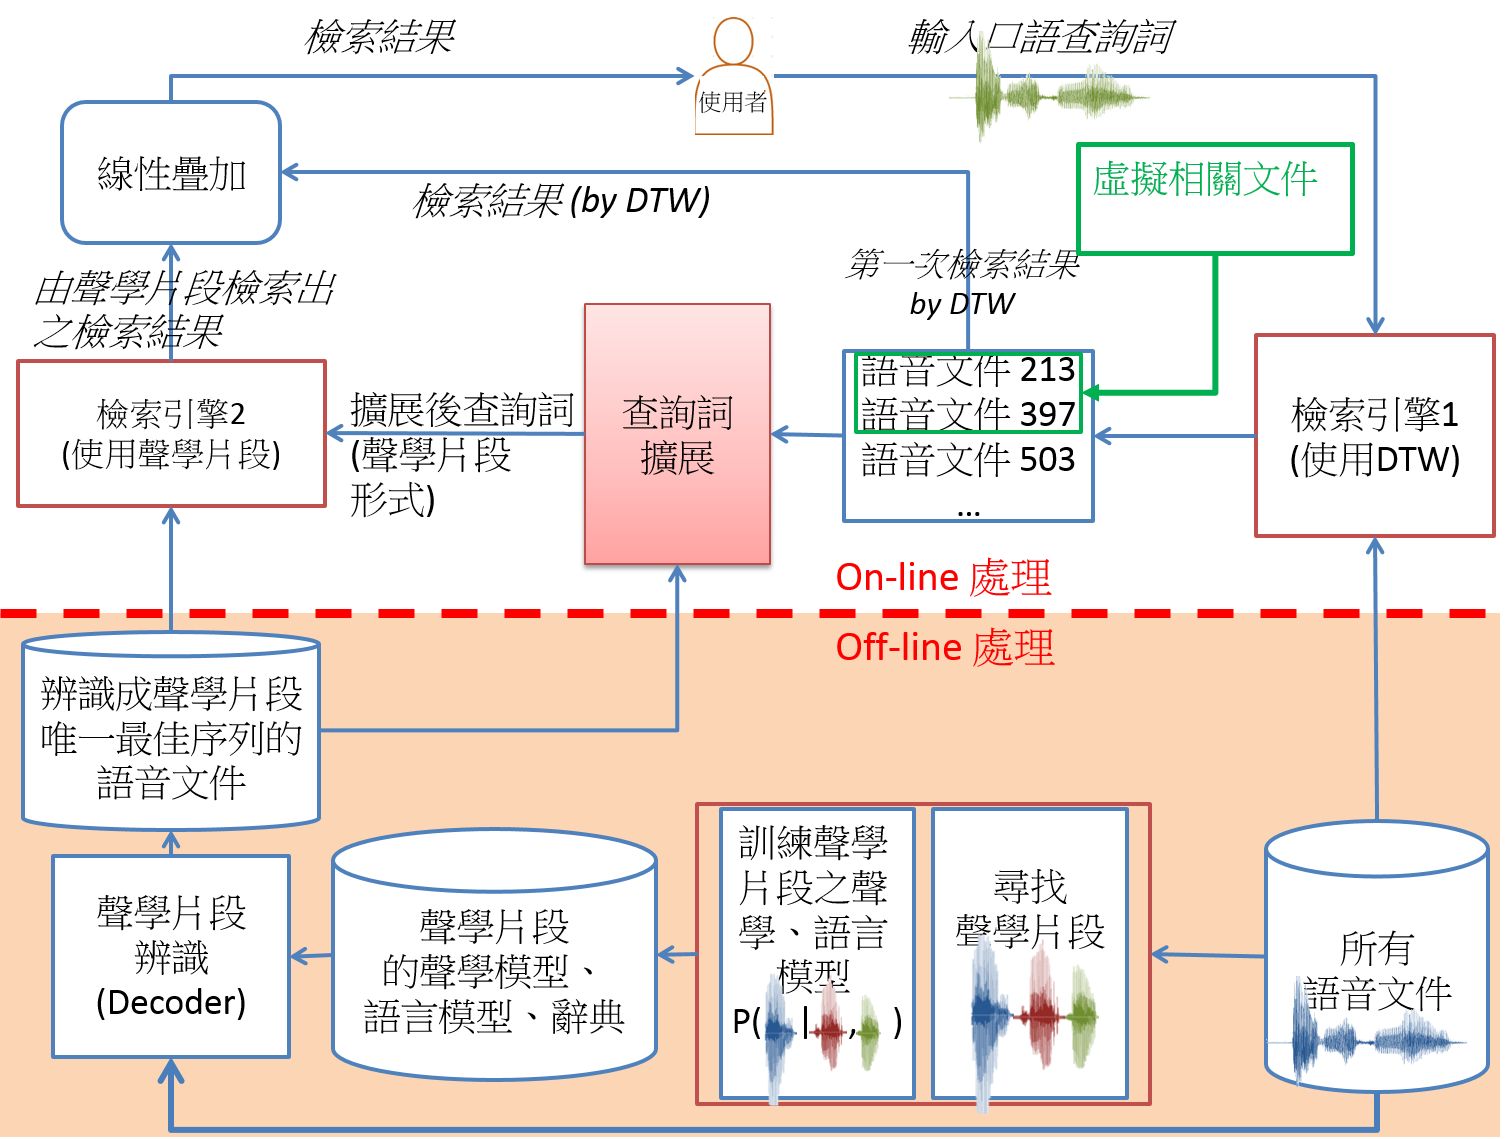
\includegraphics[scale=0.5]{images/chap4_system_zh.png}
\caption{系統架構示意圖} \label{fig:chap4_system}
\end{figure}

\subsection{前處理}
本章使用的檢索方式一樣是基於語言模型~\cite{chia2010statistical}的檢索,因此要把辨識所得的聲學片段唯一最佳序列轉換成聲學片段的語言模型,每個聲學片段唯一最佳序列 $x$ (即每個語音文件 $x$) 可以被表示為

\[
P(t|\theta_x) = \frac{C(t, x)}{\sum_t C(t, x)}
\]

$t$ 是聲學片段的標注,而 $C(t, x)$ 則是聲學片段 $t$ 在語音文件 $x$ 中出現的次數,同樣地在這裡必須將 $P(t|\theta_x)$ 與背景模型 $\theta_b$ 做平滑化,平滑化後的語音文件模型為 $\bar{\theta}_x$, $\theta_b$ 可以如下估計:

\[
P(t|\theta_b) = \frac{\sum_{x \in C} C(t, x)}{\sum_t \sum_{x \in C} C(t, x)}
\]

\subsection{第一次檢索結果}
由於使用者在此是以口述的方式輸入查詢詞,因此查詢詞是以訊號形式存在,故無法直接使用 ~\ref{sec:chap3_fpr} 提到的文字形式查詢詞的檢索,故在此處我們使用第一次檢索為 ~\ref{sec:chap4_sdtw} 提到的片段動態時間扭曲。當使用者輸入查詢詞後,系統即使用片段動態時間規劃在所有待檢索文件中找到所有的假定區域並按照相關分數排序後得到 $h_1, h_2, ...,h_n$,分別屬於語音文件 $d_1, d_2, ..., d_m$ (注意 $d_i$ 可以等於 $d_j$,因為一個語音文件中可以有多個假定區域)。將 $d_1, d_2, ..., d_m$ 去除重覆的語音文件即得第一次檢索結果。

\subsection{語意檢索}
系統至此已經得到了由片段動態時間扭曲所得的第一次檢索結果,並且可以假設其中的前 $N$ 篇為與口述查詢詞 $q$ 虛擬相關的文件,故在此試圖從這些虛擬相關的文件中找出與查詢詞 $q$ 相關的聲學片段,所採取的作法是類似 ~\ref{sec:prf}
中的查詢詞擴展的方法,只是這次不是使用在文字上,而是使用在聲學片段上,如此一來即使系統不知道那些聲學片段在文字中代表了什麼意思,但是它可以藉由觀察哪些聲學片段常常和查詢詞的聲學片段一起出現,即可將這些聲學片段當作是與查詢詞相關聯的意思。比如說如果查詢詞是口述的「美國總統」,系統不知道「美國總統」的聲音是什麼意思,但是系統會觀察到在虛擬文件中,有一些聲學片段例如「白宮」、「歐巴馬」時常與「美國總統」的聲學片段共同出現,因此即可認為「白宮」、「歐巴馬」的聲學片段是與查詢詞語意相關的,並利用「白宮」、「歐巴馬」來檢索。

\subsubsection{利用第一次檢索結果得到查詢詞}
\label{sec:chap4_decode_query}
由於查詢詞是口述形式,因此需要將查詢詞轉為聲學片段形式的語言模型,但如果直接用 ~\ref{sec:chap3_apd} 中提到的聲學片段辨識系統辨識的話,辨識結果會很差,這是由於查詢詞通常很短,而且會遇到像不同語者、不同語速和不同上下文等不匹配的問題,所以此處不會直接使用聲學辨識系統辨識,而是使用第一次檢索結果。由於第一次檢索結果會回傳查詢詞 $q$ 在虛擬相關文件中出現的假定區域,因此即可將這些假定區域對應到的唯一最佳序列中的聲學片段取出,當作口述形式查詢詞的聲學片段。

因此查詢詞模型可以如下估算:

\[
P(t|\theta_q) = \frac{\sum_{n=1}^{N} C^{'}(t, x_n)}{\sum_t \sum_{n=1}^{N} C^{'}(t, x_n)}
\]

$C^{'}(t, x_n)$ 為聲學片段 $t$ 在虛擬相關文件 $x$ 的假定區域中出現的次數。如果 $t$ 完全落在假定區域中,$C^{'}(t, x_n)$ 即為 $1$,如果只是部分落在假定區域中,$C^{'}(t, x_n)$ 即為它落在假定區域中的時間除以它自己的總長。如此一來即可得到查詢詞模型 $\theta_q$。

\subsubsection{查詢詞擴展}
此處的查詢詞擴展與 ~\ref{sec:prf} 相似,即最大化下式:
\begin{equation}
\label{equ:chap4_qe}
F_1(\phi_{qe}, \alpha_{d_1}, ..., \alpha_{d_M}) = F_1(\phi_{qe}, \alpha_{d_1}, ..., \alpha_{d_M}) F_2(\phi_{qe})^\lambda
\end{equation}
$\phi_{qe}$ 即為擴展後的聲學片段查詢詞模型,最大化上式可採用 EM 演算法,同式 ~\ref{equ:prf_estep} 與式 ~\ref{equ:prf_mstep}。

其中要特別注意的是 $F_2(\phi_{qe})$ 為:
\begin{equation}
F_2(\phi_{qe}) = \Pi_w P(w|\phi_{qe})^{P(w|\theta_q)}
\end{equation}
其中 $\theta_q$ 即為 ~\ref{sec:chap4_decode_query}中由第一次檢索結果得出的查詢詞模型。

\subsubsection{線性疊加}
有了文字的查詢詞模型與聲學片段的查詢詞模型後,即可計算查詢詞$q$與文件$x$的相關分數$S(q, x)$並排序後回傳給使用者:
\begin{equation}
\label{equ:chap4_prf_in}
S(q, x) = -[w_1 R_{DTW} (q, x) + (1-w_1) R_{QE} (q, x)]
\end{equation}
其中$R_{QE} (q, x)$為使用查詢詞擴展計算出的相關分數,$R_{DTW} (q, x)$為使用動態時間扭曲計算出的相關分數,兩者都被正規化 (Normalize) 至0和1中間。

\section{實驗設定}
\label{sec:chap4_exp_setup}
本章的實驗使用的語料為2001年間從電台廣播中錄下的4小時新聞,並手動切成5034篇語音文件,每篇語音文件大約包含了$1至3$句的語句。用來辨識的語言模型是用1999年間收集的新聞文章 (包含4000萬個詞彙) 訓練而成,辭典中包含了62000個詞彙,聲學模型是用2000年間收集的8小時廣播新聞訓練而成的音節內(Intra-syllable) 右方資訊相依(Right-context-dependent) 聲韻母模型 (Initial-Final Models)。辨識後的唯一最佳序列的字元正確率為 (Character Accuracy) 為75.27\%。
總共測試了30組查詢詞,每組查詢詞都有人工標注對應的語意相關文件,而這些語意相關文件中並「不一定要」包含查詢詞,每組查詢詞也都有人工標注的口述語彙偵測相關文件,這些文件中「一定要」包含查詢詞。本章中使用平均準確率做為評量標準。

\section{N連聲學片段分析}
\label{sec:acp_exp_setup}
前面提過了如何尋找聲學片段,此節將對找到的聲學片段進行分析,使讀者能對找到的聲學片段有更實際的了解。在這章中,我們將 5034 句的新聞語音文件辨識成兩階段的聲學片段,包括字單位與詞單位的聲學片段,系統總共從目標語料庫中找到了 208 個字單位的語音片段,並使用這些字單位聲學片段的單聯 (Unigram) 、雙聯 (Bigram) 和三聯 (Trigram) 組合 (總共 85534 個組合) 來表示每一個語音文件模型 ($\theta_x$) 與查詢詞模型 ($\theta_Q$)
並用在檢索系統當中。大多數的字單位語音片段接近中文的音節,所以雙聯、三聯組合則接近於中文的雙音節詞或是三音節詞。表 ~\ref{table:chap4_pattern_example} 中列了一些語音片段與其對應到的聲音和含義,比如說第 (1) 列中的是單聯聲學片段 (其聲學片段編號為106),它的聲音是 /dian/ ,但由於同樣的聲音在中文中可以對應到很多的意思,因此這裡其中的幾個如「店」、「點」、「電」等。第 (2) 列中的是一個雙聯聲學片段 (由兩個編號為 (106) 和 (27) 的聲學片段組成)
,其對應到的意思是「電腦」、「電能」等,由於這裡是將類似聲音的字分群在一起,因此有些實際上讀音未必一樣但很像的詞也會被分群在一起。

\begin{table}[htbp]
%\resizebox{\columnwidth}{!}{
\centering
\begin{tabular}{|lll|}
\hline
 & $t$ (n連聲學片段): (IDs) & 聲學片段範例 \\
\hline
 & &  店(/dian/), \\
(1) & 單聯: (106) & 點(/dian/), 電(/dian/) \\
\hline 
 &  & 電腦(/dian-nau/), \\
(2) & 雙連: (106)-(27) & 電能(/dian-neng/) \\
\hline
 & & 手(/shou/), \\
(3) & 單連: (93) &  收(/shou/), 熟(/shou/)\\ 
\hline
 & & 受傷(/shou-shang/), \\
(4) & 雙連: (93)-(145) &  首相(/shou-shiang/) \\
\hline

\end{tabular}
%}
\caption{一些單聯和雙聯聲學片段的聲音與其對應到的中文詞}
\label{table:chap4_pattern_example}
\end{table}



\section{實驗結果及分析}
表 ~\ref{table:chap4_result1} 中列出了本章提出的檢索方法的結果。列 (1) 中的結果是只有第一次檢索結果 (即圖 ~\ref{fig:chap4_system} 中的檢索引擎1),列(2) 中的結果是圖 ~\ref{fig:chap4_system} 中的檢索引擎2,為只使用查詢詞擴展後的結果,列 (3) 中顯示了將兩者以不同權重 $w_1$ 線性疊加後的結果。欄 (A) 中是用語意檢索的答案計算出的平均準確率,也就是說欄 (A) 中的答案都是與查詢詞語意上相關而且不一定要包含查詢詞的文件,欄 (B)
是用有出現查詢詞的文件當作答案,因此欄 (B) 的平均準確率都會比欄 (A) 高上許多。雖然欄 (A) 中的平均準確率都低於 $ 10\% $,但這是由於語意檢索與生俱來的困難性和聲學片段模稜兩可的特性所致。首先在欄 (A) 中可以觀察到本章提出的查詢詞擴展能夠有效地幫助到非監督式語意檢索 (列(3)
對比列(1)),多半是由於查詢詞擴展能夠有效地從第一次檢索結果中找出與查詢詞語意相關的資料。很有趣的是本章的查詢詞擴展也能有效地幫助到口述語彙檢索的結果(欄(B)),可能是因為動態時間扭曲在比對查詢詞與文件時,很有可能會因為信號的不匹配 (Signal mismatch)
如語速、語者、發音等聲學差異而使得動態時間扭曲比對錯誤,但查詢詞很有可能會常與某些詞一起出現,一旦系統透過查詢詞擴展將這些常與查詢詞一起出現的詞加入擴展後查詢詞中,系統即可利用這些常一起出現的詞去找到擁有查詢詞的文件。由表 ~\ref{table:chap4_result1} 中可以注意到系統對於線性疊加的權重$w_1$並不是很敏感,在$w_1=0.7$和$w_1=0.9$都可以觀察到進步,由於$w_1=0.7$是最好的結果,因此在後續的實驗會將$w_1$設為$0.7$。

同時我們也想比較監督式的查詢詞擴展(~\ref{sec:chap4_semantic_retrieval}節)在語意檢索上和口述語彙偵測的結果,這些結果呈現在表 ~\ref{table:chap4_result1} 的下半部,這結果是先將所有的語音文件辨識成文字轉寫,再利用文字形式的查詢詞進行查詢詞擴展的檢索,在這邊可以觀察到查詢詞擴展在監督式的查詢下能有效地使系統進步 (列(6)(7))。可以觀察到監督式的語意檢索進步量約為 $1.28\%$,而非監督式的語意檢索可以達到 $0.94\%$ 的進步量,而這進步量是接近於已被驗證許久的監督式查詢詞擴展了。

% Table generated by Excel2LaTeX from sheet '工作表1'
\begin{table}[htbp]
  \centering    
  %\resizebox{\columnwidth}{!}{     

    \begin{tabular}{|l|l|l|c|c|}
    \hline
    \multicolumn{3}{|l|}{} & \multicolumn{1}{l|}{(A)} & \multicolumn{1}{l|}{(B)} \\
    \multicolumn{3}{|l|}{} & \multicolumn{1}{l|}{} & \multicolumn{1}{l|}{口述} \\
    \multicolumn{3}{|l|}{平均準確率} & \multicolumn{1}{l|}{語意檢索} & \multicolumn{1}{l|}{詞彙偵測} \\
    \hline

    \multirow{5}[2]{*}{\begin{sideways}非監督式檢索~~ \end{sideways}} & \multicolumn{2}{l|}{(1) 第一次檢索結果(DTW) ($w_1=1.0$)} & 8.76\% & 28.30\% \\
    \cline{2-5} 
\cline{4-5}          & \multicolumn{2}{l|}{(2) 查詢詞擴展 ($w_1=0.0$)} & 6.03\% & 7.82\% \\
\cline{2-5}          & \multirow{2}[4]{*}{(3) 線性疊加} & $w_1=0.9$ & 9.28\% & 29.94\% \\
\cline{3-5}          &       & $w_1=0.7$ & 9.70\% & 30.31\% \\
\cline{2-5}          & \multicolumn{2}{l|}{(4) 進步量 ($w_1=0.7$)} & 0.94\% & 2.01\% \\
    \hline
    \multirow{4}[8]{*}{\begin{sideways} ~~~~~~監督式檢索 \end{sideways}} & \multicolumn{2}{l|}{(5) 第一次檢索結果 ($w_1=1.0$)} & 29.49\% & 70.07\% \\
\cline{2-5}          & \multicolumn{2}{l|}{(6) 查詢詞擴展 ($w_1=0.0$)} & 30.30\% & 68.86\% \\
\cline{2-5}          & \multicolumn{2}{l|}{(7) 線性疊加 ($w_1=0.7$)} & 30.77\% & 76.80\% \\
\cline{2-5}          & \multicolumn{2}{l|}{(8) 進步量} & 1.28\% & 6.73\% \\
    \hline
    \end{tabular}%

  %  }
  \caption{系統在語意檢索和口述語彙偵測時的平均準確率}
  \label{table:chap4_result1}%

\end{table}%

接著我們想觀察本章提出的方法是否真的能找到更多語意上相關的文件。首先,在使用動態時間扭曲產生第一次檢索結果時,對於每個查詢詞都取出其相關分數最高的200篇文件,由於總共有30個查詢詞,因此總共有6000篇文件,此為表 ~\ref{table:chap4_result2} 中的列(1),利用本章方法找出的6000篇文件為列 (2),欄 (A) 中為這6000篇文件中與查詢詞語意相關的文件數,欄 (B) 為欄 (A)中有出現查詢詞的文件數,欄 (C)為欄 (A)中沒有出現查詢詞的文件數,從表中可以看到,本章的方法確實能夠找到更多語意相關但是不包含查詢詞的文件,進步量為$15.07\%$,而這些文件通常是很難被找到的,另外欄 (A) 和欄 (C) 中也各有 $13.41\%$ 和 $11.36\%$ 的進步。

\begin{table}[htbp]
  \centering
    \resizebox{\columnwidth}{!}{     

    \begin{tabular}{|l|c|c|c|}
    \hline
          & (A) 所有與 & (B)          & (C)  \\
    MAP   & 查詢詞語意 & (A) 中不含查 & (A) 中含查  \\
          & 相關的文件 & 詢詞的文件   & 詢詞的文件 \\
    \hline
    (1) 第一次檢索結果 (DTW) & \multirow{2}[4]{*}{589} & \multirow{2}[4]{*}{325} & \multirow{2}[4]{*}{264} \\
   ($w_1=1.0$) &       &       & \\
    \hline
    (2) 本章提出的方法 & \multirow{2}[4]{*}{668} & \multirow{2}[4]{*}{374} & \multirow{2}[4]{*}{294} \\
  ($w_1=0.7$) &       &       & \\
    \hline
    (3) 進步量 & 13.41\% & 15.07\% & 11.36\% \\
    \hline
    \end{tabular}%
    }
    \caption{系統找回與查詢詞語意相關的文件數量,包括含查詢詞與不含查詢詞的文件數。}
    \label{table:chap4_result2}%
\end{table}%

接著來觀察系統的參數$N$(虛擬相關文件數)、$w_1$(式 ~\ref{equ:chap4_prf_in} 中線性疊加的權重) 和$\lambda$(式~\ref{equ:chap4_qe}中原查詢詞模型對於查詢詞擴展時的影響)對於系統的影響。圖 ~\ref{fig:chap4_resulta} 和圖 ~\ref{fig:chap4_resultb} 中顯示了使用不同的線性疊加權重 $w_1$ 時系統的平均準確率,縱軸為平均準確率 (MAP),橫軸為不同的線性疊加權重 $w_1$, 圖中使用的答案均為語意檢索的答案,圖中的紅色虛線為檢索系統的基準 (Baseline) 檢索結果,為使用動態時間扭曲產生的第一次檢索結果。圖 ~\ref{fig:chap4_resulta} 中固定 $N$ 為 $12$,將$\lambda$改變為$0,
300, 900, 1500$,可以觀察到當$\lambda = 0$時,系統的表現是特別差的,因為此時系統會過適到虛擬相關文件的主題中,當$\lambda>300$後,系統的表現並不隨$\lambda$改變而影響太多,而最好的表現出現於$\lambda=300$,另外可以注意到系統在$w_1$從$0.45$到$0.95$時都有進步,因此本系統對於$w_1$的改變並不是太敏感。
圖 ~\ref{fig:chap4_resultb} 中將 $\lambda$ 固定為 $300$,並改變 $N$為 $4, 12, 20, 32, 64$。同樣地可以觀察到 $w_1$ 從$0.45$到$0.95$都有進步,並且當$N$上升時,平均準確率會先上升後下降,這原因是當$N$上升時,有更多文件被當作虛擬相關文件,因此有更多的訓練資料,但當$N$太大時,系統會用過多的不相關資料訓練,進而使得系統的表現下降。

\begin{figure}
\centering
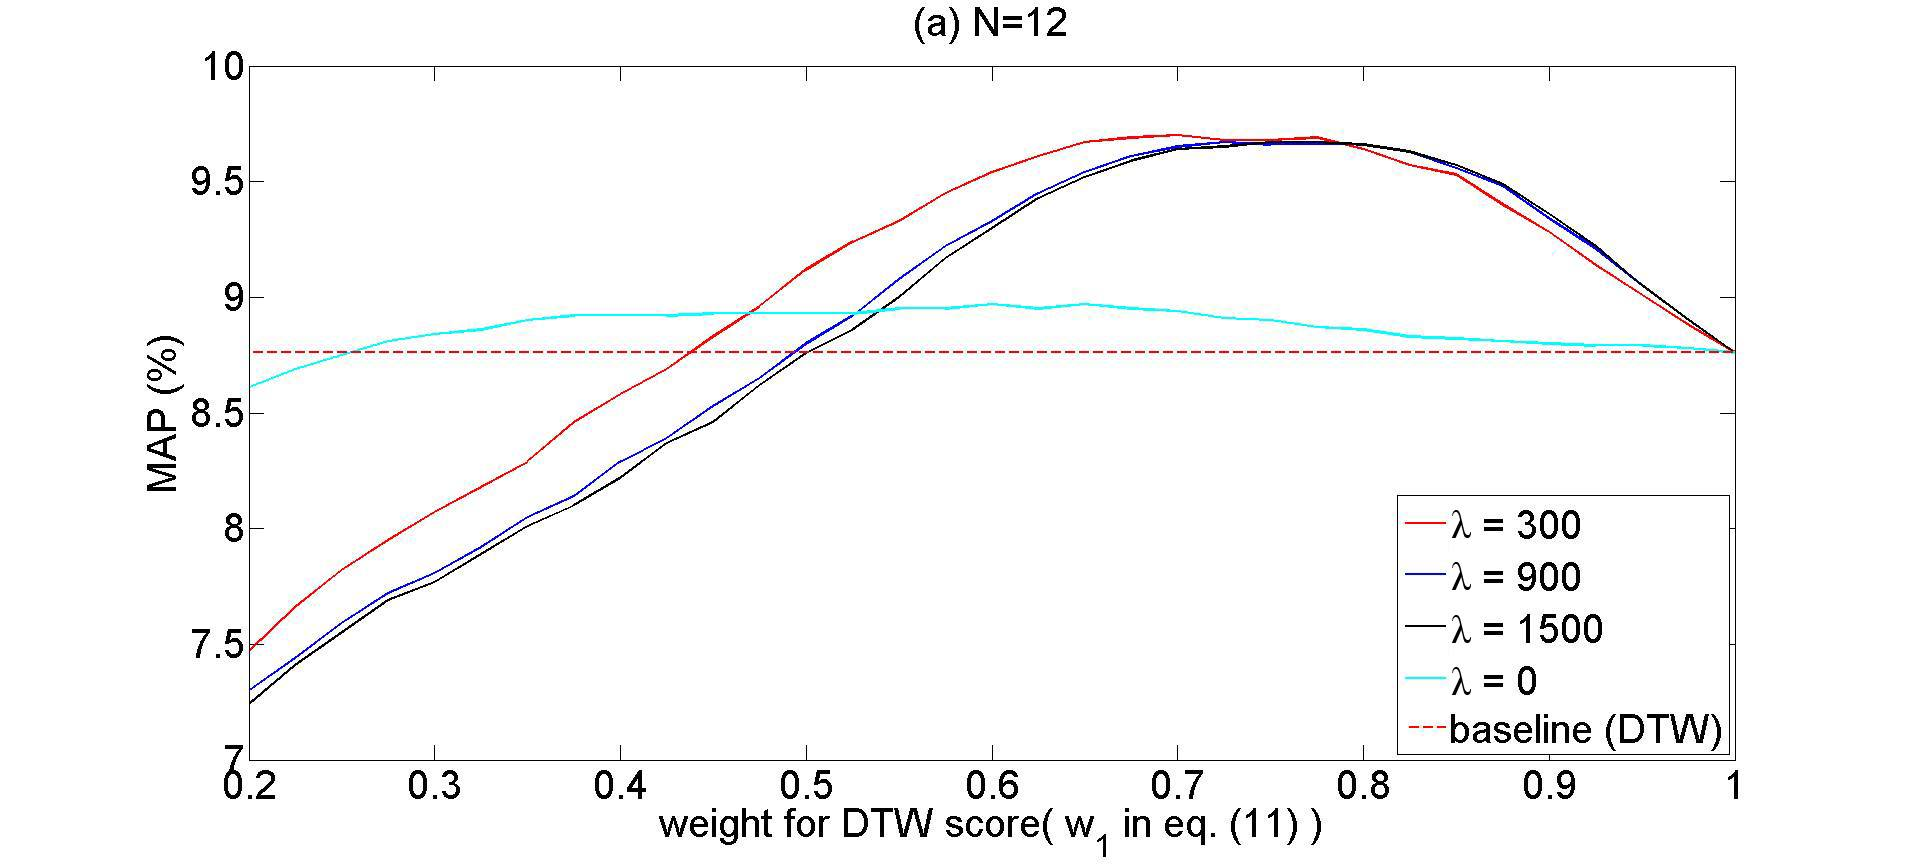
\includegraphics[scale=0.18]{images/chap4_resulta.jpg}
\caption{將第一次檢索結果和聲學片段形式的查詢詞擴展檢索結果疊加後的平均準確率 $(N = 800)$} \label{fig:chap4_resulta}
\centering
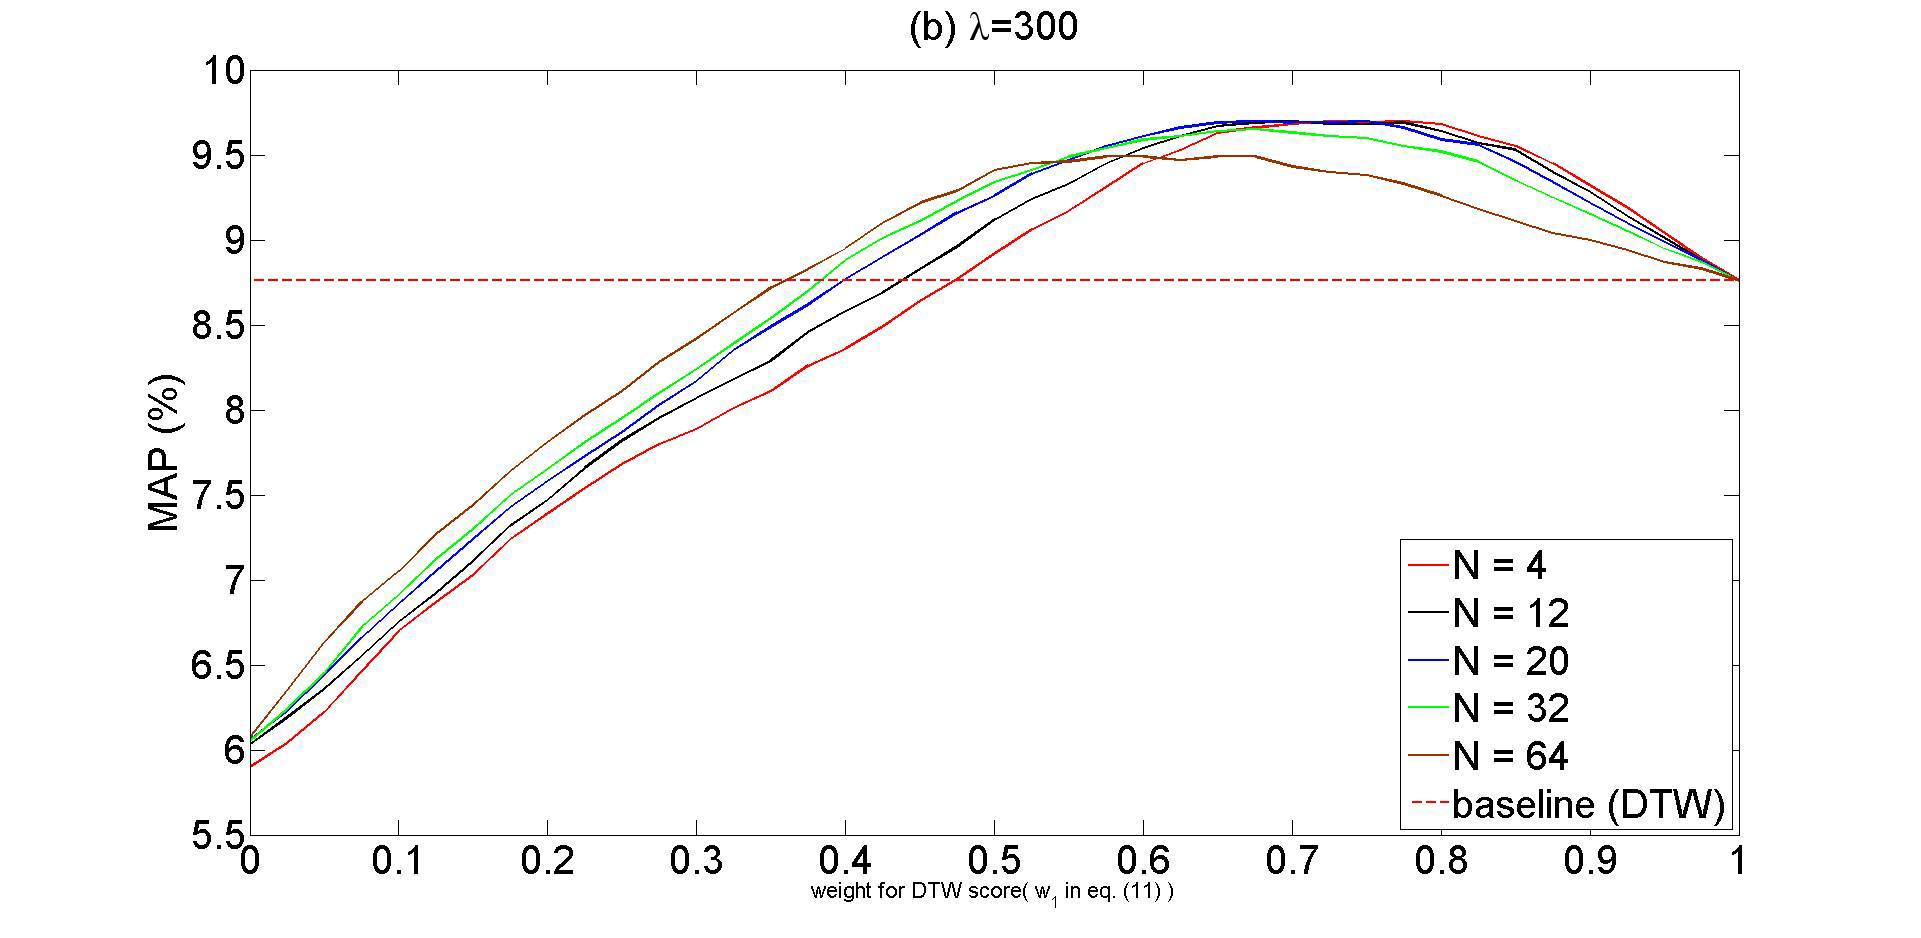
\includegraphics[scale=0.18]{images/chap4_resultb.jpg}
\caption{將第一次檢索結果和聲學片段形式的查詢詞擴展檢索結果疊加後的平均準確率 ($\lambda = 300$)} \label{fig:chap4_resultb}
\end{figure}


\subsection{聲學片段語意檢索能力分析}
表 ~\ref{table:chap4_spa} 中的實驗顯示了本章提出的方法確實能夠在聲學片段的查詢詞中加入與查詢詞語意相關的聲學片段,即使系統並不知道這些聲學片段的含義。表 ~\ref{table:chap4_spa} 中是「學校」這個查詢詞在經過本章的查詢詞擴展後機率 $P(t|\theta_Q)$ 最高的五個N聯聲學片段。列 (1)(2) 中的聲學片段為 ~\ref{sec:chap4_decode_query}
中提到的利用第一次檢索結果得到的原查詢詞的聲學片段,很明顯地列 (1)(2) 中的聲學片段在擴展後的查詢詞模型中也佔了大部分的機率。列 (3)(4)(5) 中的N聯聲學片段則是在查詢詞擴展的過程中被自動加進去的,列 (3) 是由列 (1)(2) 中的單連聲學片段組合而成的雙連聲學片段,列 (4) 中的單聯聲學片段對應到的中文聲音其實是與列 (2) 中非常相似,但由於訓練時因為聲學上的特徵不一樣而被分群為不同的聲學片段,在此本章的方法也能將這些片段加進來進而提升檢索結果。而列 (5) 加進來的是雙連聲學片段,對應到的中文為「學生」,而這是與查詢詞「學校」有語意相關的詞,因此被系統加進來後也能提升檢索的結果。由以上的觀察可以發現本章提出的方法確實能把與查詢詞語意相關的聲學片段加進查詢詞模型中,並達成非監督式語意檢索。

\begin{table}[htbp]
\centering
%\resizebox{\columnwidth}{!}{     
\begin{tabular}{llll}
\hline
& $t$(n連聲學片段): (IDs) & $P(t|\theta_Q)$ & 範例聲學片段 \\
\hline 
(1) & 單連: (87) & 0.4280 & 校(/xiao/) \\
(2) & 單連: (56) & 0.3880 & 學(/xue/) \\
(3) & 雙連: (56)-(87) & 0.0040 & 學校(/xue-xiao/) \\
(4) & 單連: (129) & 0.0030 & 學(/xue/) \\ 
(5) & 雙連: (129)-(23) & 0.0016 & 學生(/xue-sheng/) \\
\end{tabular}
%}
\caption{查詢詞為"學校(/xue-xiao/)"時,擴展後查詢詞模型 $\phi_{qe}$中機率最大的五組聲學片段}
\label{table:chap4_spa}
\end{table}

\section{本章總結}
本章嘗試了使用聲學片段完成了非監督式的語意檢索,使用此種方法即可在不需要人為標注的情況下達成語意檢索。如此一來即不需要花費很多時間、金錢完成人為標注,不過目前非監督式語意檢索的表現比起監督式仍有一段落差,仍然需要更多的研究才能夠使其應用在產業中。
